\section{Testing and Benchmarking}

\begin{frame}
	\frametitle{Benchmarking vs Testing}
	\begin{itemize}
		\item \textbf{Benchmarking} will give you system-wide metrics for:
			\begin{itemize}
				\item Your hardware platform
				\item Your Kernel configuration
				\item Your Non-critical userspace stack
			\end{itemize}
		\item \textbf{Testing} will ensure that your business application behaves correctly
		\item Stressing tools used for benchmarking can also be used for testing
		\item It's important to always consider the \textbf{Worst Case Scenario}
	\end{itemize}
\end{frame}

\begin{frame}
  \frametitle{ftrace - Kernel function tracer}

  Infrastructure that can be used for debugging or analyzing latencies
  and performance issues in the kernel.

  \begin{itemize}
  \item Very well documented in \kdochtml{trace/ftrace}
  \item Negligible overhead when tracing is not enabled at run-time.
  \item Traces \textbf{events}, defined within the kernel code, in \textbf{per-cpu buffers}
  \item Events have associated context:
	  \begin{itemize}
		  \item \code{sched:sched_switch} : Context switch, indicates \code{prev_pid}, \code{next_pid}
	  \end{itemize}
  \item Can also be used to trace any kernel function with the \textbf{function tracer}
  \end{itemize}
\end{frame}

\begin{frame}
  \frametitle{Using ftrace}
  \begin{itemize}
  \item Tracing information available through the \code{tracefs} virtual fs
  \item Mount this filesystem as follows:\\
    \code{mount -t tracefs nodev /sys/kernel/tracing}
  \item On some systems, it can also be found in \code{/sys/kernel/debug/tracing}
  \item Check available tracers:
	  \begin{itemize}
		  \item \code{cat /sys/kernel/tracing/available_tracers}
	  \end{itemize}
  \item Select the interesting events:
	  \begin{itemize}
		  \item \code{echo 1 > /sys/kernel/tracing/events/[X/Y/]enable}
	  \end{itemize}
  \item Start/stop tracing:
	  \begin{itemize}
		  \item \code{echo [0|1] > /sys/kernel/tracing/tracing_on}
	  \end{itemize}
  \item Retrieve the trace:
	  \begin{itemize}
		  \item \code{/sys/kernel/tracing/trace}: The trace buffers merged
		  \item \code{/sys/kernel/tracing/trace_pipe}: Stream the trace buffers, consuming data
		  \item \code{/sys/kernel/tracing/per-cpu/cpuX/trace}: Per-cpu traces
	  \end{itemize}
  \end{itemize}
\end{frame}

\begin{frame}[fragile]
  \frametitle{Scheduling latency tracer}
  \fontsize{9}{9}\selectfont
  \kconfig{CONFIG_SCHED_TRACER} ({\em Kernel Hacking} section)
  \begin{itemize}
  \item Maximum recorded time between waking up a top priority task
    and its scheduling on a CPU, expressed in us.
  \item Check that \code{wakeup} is listed in
    \code{/sys/kernel/tracing/available_tracers}
  \item To select, reset and enable this tracer:
    \begin{block}{}
\begin{verbatim}
echo wakeup > /sys/kernel/tracing/current_tracer
echo 0 > /sys/kernel/tracing/tracing_max_latency
echo 1 > /sys/kernel/tracing/tracing_enabled
\end{verbatim}
    \end{block}
  \item Let your system run, in particular real-time tasks.\\
    Dummy example: \code{chrt -f 5 sleep 1}
  \item Disable tracing:\\
    \begin{block}{}
\begin{verbatim}
echo 0 > /sys/kernel/tracing/tracing_enabled
\end{verbatim}
    \end{block}{}
  \item Read the maximum recorded latency and the corresponding trace:\\
    \begin{block}{}
\begin{verbatim}
cat /sys/kernel/tracing/tracing_max_latency
\end{verbatim}
    \end{block}{}
  \end{itemize}
\end{frame}

\begin{frame}
	\frametitle{trace-cmd}
	\begin{itemize}
		\item Wrapper around the \code{ftrace} interface
		\item Trace only during a program execution:
			\begin{itemize}
				\item \code{trace-cmd record <opts> <cmd>}
				\item \code{trace-cmd report}
			\end{itemize}
		\item Start, stop and show the trace buffer:
			\begin{itemize}
				\item \code{trace-cmd start <opts>}
				\item \code{trace-cmd stop}
				\item \code{trace-cmd show}
			\end{itemize}
		\item Save the content of the trace buffer for further analysis:
			\begin{itemize}
				\item \code{trace-cmd extract}
			\end{itemize}
		\item Options
			\begin{itemize}
				\item Events: \code{-e sched}, \code{-e sched:sched_switch}
				\item Plugins: \code{-p function}
				\item Tracers: \code{-t osnoise}
				\item Functions: \code{-f netif_tx_wake_queue}
			\end{itemize}
	\end{itemize}
\end{frame}

\begin{frame}
	\frametitle{rtla}
	\textbf{R}eal\textbf{T}ime \textbf{L}inux \textbf{A}nalysis tool
	\begin{itemize}
		\item Developped by Daniel Bristot de Oliveira
		\item High-level interface to the \code{timerlat} and \code{osnoise} tracers
		\item \code{rtla osnoise|timerlat top|hist} gives high-level view of noise and latencies
		\item Can generate histograms, that can then be visualized
	\end{itemize}

\end{frame}

\begin{frame}
	\frametitle{rtla - osnoise}
	\begin{itemize}
		\item Gives an overview of "noise" sources from the Kernel and the Hardware
		\item Uses a similar measurement loop as \code{hwlatdetect}
		\item Uses \code{tracepoints} to detect the source of noise:
			\begin{itemize}
				\item Thread Latency: Latencies due to the measuring thread being preempted
				\item SoftIRQ Latency: Latencies due to softIRQ processing
				\item IRQ Latency: Latencies introduced by IRQs
				\item NMI Latency: Latencies introduced by NMIs
				\item Hardware Latency: Latencies that aren't explained by any of the above
			\end{itemize}
		\item \code{trace-cmd start -p osnoise}: Start recording os noise events
		\item \code{trace-cmd start -p osnoise -e osnoise}: Start recording noise events and trace their cause
	\end{itemize}
\end{frame}

\begin{frame}
	\frametitle{rtla - timerlat}
	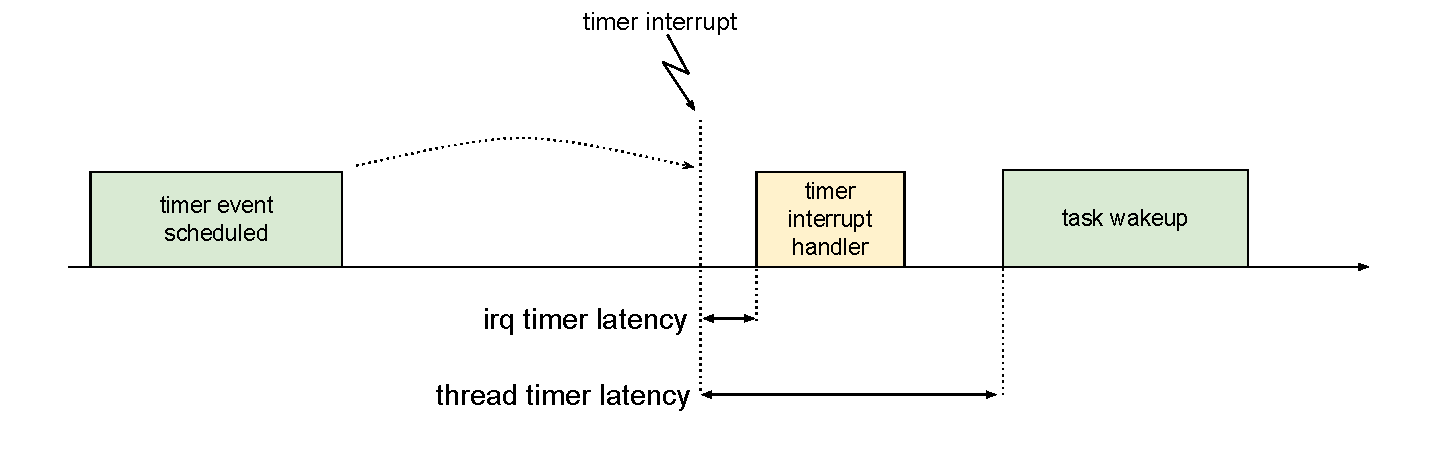
\includegraphics[width=\textwidth]{slides/realtime-linux-benchmarking/rtla.pdf}
	\begin{itemize}
		\item Periodic, per-cpu wakeup latency measurement in-kernel
		\item Can differentiate the IRQ wakeup time from the scheduling wakeup time
		\item Can use \code{osnoise} tracepoints to analyze the delay sources
		\item Can also trace \textbf{User return} latency, to benchmark custom applications
	\end{itemize}
	%%% Schematics
\end{frame}

\begin{frame}
	\frametitle{rtla autoanalysis}
	\begin{itemize}
		\item Running \code{timerlat -a <us>} will trigger the auto-analysis mode
		\item A threshold is set with \code{-a}
		\item Measurement will stop if a latency higher than the threshold is detected
		\item Timerlat then prints a stack trace with the cause of the latency
		\item Can identify if the latency comes from a \textbf{blocking} or an \textbf{interference}
		\item Can identify the \textbf{task} of \textbf{interrupt} at the origin of the latency
		\item Can identify if the \textbf{hardware} itself is the culprit
	\end{itemize}
\end{frame}

\begin{frame}
	\frametitle{rtla - hwnoise}
	\begin{itemize}
		\item Focus on Hardware-induced latencies
		\item Similar to osnoise, but runs with \textbf{interrupts disabled}
		\item Only the hardware or non-maskable interrupts can interfere with measurements
		\item Tries to assign the noise to \code{NMI} when it can
		\item \textbf{NMI-based} watchdogs and \textbf{Hyperthreading} can cause such latencies
	\end{itemize}
\end{frame}

\begin{frame}
	\frametitle{kernelshark}
	\begin{itemize}
		\item Kernelshark is a graphical interface for processing ftrace reports
		\item It's better used with \code{trace-cmd}, an interface to ftrace
		\item Useful when a deep analysis is required for a specific bug 
		\item \code{trace-cmd list}
		\item \code{trace-cmd record -e <event> [<command>]}
		\item \code{kernelshark}
	\end{itemize}
\end{frame}

\begin{frame}
	\frametitle{hwlatdetect}
	Tool provided by \code{rt-tests}, relying on a dedicated \code{ftrace} tracer.
	\begin{itemize}
		\item Predecessor to \textbf{rtla hwnoise}
		\item Runs a tight loop on all CPU cores with local interrupts disabled
		\item Only NMIs and Hardware Latencies can interrupt the loop
		\item Samples a high precision timer and looks for large gaps between samples
		\item Useful to benchmark and validate a hardware platform
		\item Must \textbf{not} be used in production environment, introduces huge latencies
	\end{itemize}
\end{frame}



\begin{frame}
	\frametitle{cyclictest}
	\begin{itemize}
		\item Tool that tests the System and Kernel Latencies
		\item Provided by the \code{rt-test} suite
		\item Schedules timer events and compares the expected and actual wakeup time
		\item Measures the kernel-induced latencies, but also hardware-induced latencies
		\item Can create graphs, and be used with tracing subsystems
		\item Best used in conjunction with various stressing workloads
		\item Should be run for long amounts of time
	\end{itemize}
\end{frame}

\begin{frame}
	\frametitle{hackbench}
	Stress and benchmark the Linux Kernel Scheduler
	\begin{itemize}
		\item Stresses the scheduler by creating lots of processes of threads
		\item They communicate with each-other through sockets or pipes
		\item This generates lots of context switches and scheduling events
		\item Useful to check how a RT program behaves when heavy workloads run in parallel
	\end{itemize}
\end{frame}

\begin{frame}
	\frametitle{stress-ng}
	Very feature-full stressing utility, with more than 260 stressors
	\begin{itemize}
		\item Can stress very specific aspects of the system:
			\begin{itemize}
				\item Specific syscalls
				\item CPU instructions and computations
				\item Caches, Memory access, Page-faults
				\item Network and Filesytem stacks
			\end{itemize}
		\item Very useful to accurately simulate known workloads
	\end{itemize}
\end{frame}

\begin{frame}
	\frametitle{rteval}
	\begin{itemize}
		\item Allows orchestrating stressing tools and testing tools
		\item Loads are \textbf{hackbench}, \textbf{kcompile} and \textbf{stress-ng}
		\item Testing tools are \textbf{cyclictest} and \textbf{timerlat}
		\item Describe a full test through configuration files
		\item Generates a test report
		\item Ideal to integrate in a CI environment
	\end{itemize}
	\url{https://git.kernel.org/pub/scm/utils/rteval/rteval.git/}
\end{frame}

\subsection{Benchmarking an application}
\begin{frame}
	\frametitle{strace}
	strace is a userspace tool that trace system-calls and signals
	\begin{itemize}
		\item Help analyze how an application interacts with the kernel
		\item Some syscalls can be detrimental to RT behaviour
		\item strace can help understand what an application does
		\item Helpful for external libraries
	\end{itemize}
\end{frame}

\begin{frame}
	\frametitle{perf}
	perf is a performance analysis tool that gathers kernel and hardware statistics
	\begin{itemize}
		\item Uses Hardware Counters and monitoring units
		\item Uses Kernel Counters and the tracing infrastructure
		\item Can profile the whole system, an application, a CPU core, etc.
		\item Very versatile, but tied to the kernel version
		\item Perf relies on various \textbf{events} reported by the kernel
	\end{itemize}
\end{frame}

\begin{frame}
	\frametitle{Using perf, examples}
	\begin{itemize}
		\item Lots of events measurable: hardware events, software events, cache misses, power management
			\begin{itemize}
				\item \code{perf list}
			\end{itemize}
		\item Display statistics in real-time
			\begin{itemize}
				\item \code{perf top}
				\item \code{perf top -e cache-misses}
				\item \code{perf top -e context-switches}
			\end{itemize}
		\item Investigate scheduling latencies
			\begin{itemize}
				\item \code{perf sched record}
				\item \code{perf sched latency}
			\end{itemize}
	\end{itemize}
\end{frame}

\begin{frame}
	\frametitle{Other useful tools}
	\begin{itemize}
		\item \code{vmstat}: Displays the system state, interrupts, context switches...
			\begin{itemize}
				\item \code{vmstat -w 0}
			\end{itemize}
		\item \code{powertop}: Display the CPU usage
		\item \code{cat /sys/kernel/realtime}: Indicates if the RT Patch is applied
		\item \code{htop}: Displays running tasks, including kernel tasks
	\end{itemize}
\end{frame}

